\documentclass{article}
% \usepackage{xeCJK}
\usepackage{amsmath}
\usepackage{amssymb}
\usepackage{mathrsfs}
\usepackage{xcolor}
\usepackage{bm}
\usepackage{hyperref}
\usepackage{graphicx}
\usepackage{subcaption}
\usepackage{float}
\usepackage{multicol}
\usepackage{pdfpages}
\usepackage[ruled,linesnumbered]{algorithm2e}

\bibliographystyle{plain}
\setlength{\parindent}{2em}
\usepackage{geometry}
\geometry{a4paper, left=2.54cm, right=2.54cm, top=3.18cm, bottom=3.18cm}

% set line spacing
% \renewcommand{\baselinestretch}{1.5}

% define reference format
\hypersetup{
    colorlinks=true,
    linkcolor=blue,
    urlcolor=blue,
    citecolor=blue,
    linkbordercolor=white
}

\title{\textbf{Chemotactic Network Designing}}
\author{Yichen Lu}

\begin{document}

\maketitle

\tableofcontents

\newpage
\section{Models}

\subsection{Thinking Process}

\begin{subequations}
    \begin{align}
        &\dot{\mathbf{r}}_i\left( t \right) =\alpha_c \nabla c-\nabla _{\mathbf{r}_i}V+\sqrt{2D_p}\boldsymbol{\eta }_i\\
        &\dot{c}\left( \mathbf{r},t \right) =D_c\nabla ^2c-k_cc+\beta _c\sum\nolimits_j^{}{\delta \left( \mathbf{r}-\mathbf{r}_{j}^{*} \right)}
    \end{align}
\end{subequations}
for $i=1,2,\cdots,N$ and $j=1,2,\cdots,M$. Here, $\mathbf{r}_i, \mathbf{r}_j^*$ is the position of the $i$-th particle, $j$-th target node, respectively, $c$ is the concentration of the signal chemical released by the node, $\alpha _c<0$ is the chemotactic sensitivity, $V$ is the potential field of short-range repulsion, $D_p$ is the intensity of thermal noise, $s_i$ is the internal state of the $i$-th particle, $D_c$ is the diffusion coefficient, $k_c$ is the decay rate of the chemical, and $\beta _c$ is the production rate of the target nodes. 

\begin{figure}[htbp]
    \centering
    \subcaptionbox{Horizontal distance of nodes $d_n=7$}[0.49\linewidth]{
      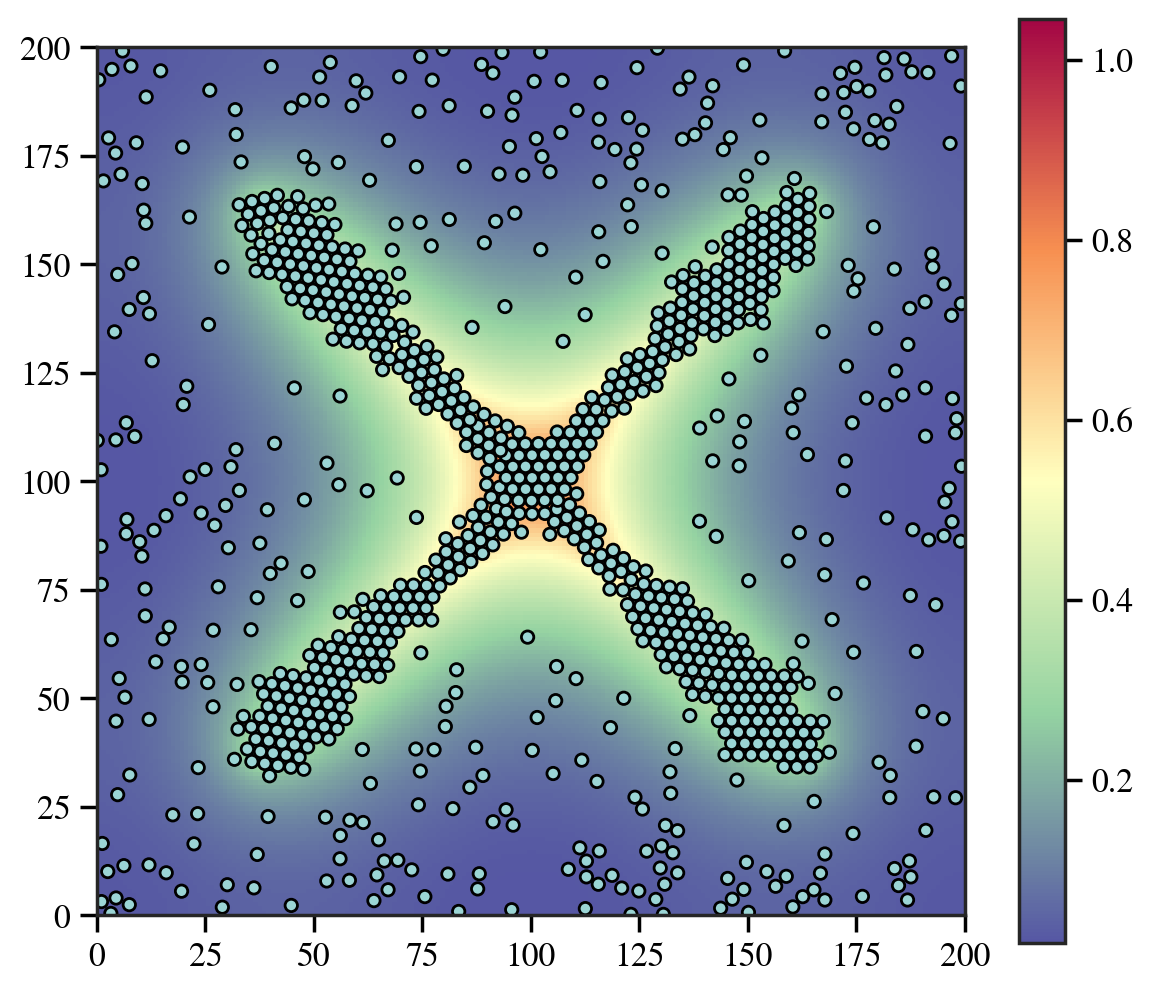
\includegraphics[width=\linewidth]{figs/simpleModeling1.png}
    }
    \hfill
    \subcaptionbox{$d_n=10$}[0.49\linewidth]{
      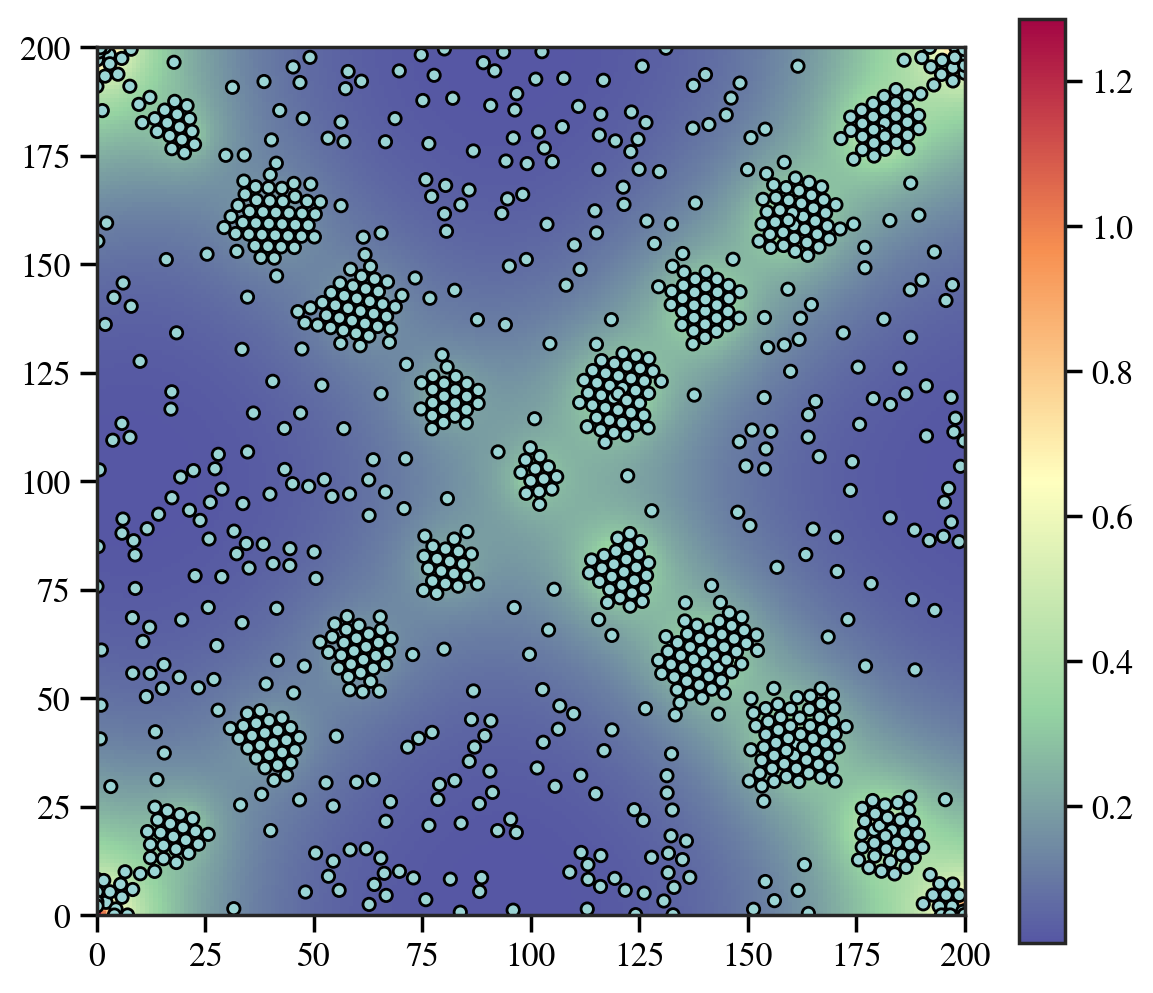
\includegraphics[width=\linewidth]{figs/simpleModeling2.png}
    }
    \caption{
        The simulation of the above model with $\alpha_c=-5$, $D_c=2$, $k_c=0.001$ and $\beta_c=0.3$. When the horizontal distance of nodes $d_n$ is small, the nodes are connected by the particles. While, when $d_n$ is large, the particles are not connected. 
    }
\end{figure}

% Introduce adaptive dynamics to the particles by incorporating a new variable, $s_i$, representing the internal state of the $i$-th particle, which governs its sensitivity to the chemical signal. Additionally, assume that the particles can modulate the local chemical concentration but do not actively produce the chemical. The updated model is as follows:
% \begin{subequations}
%     \begin{align}
%         &\dot{\mathbf{r}}_i\left( t \right) =\alpha _c\nabla c-\nabla _{\mathbf{r}_i}V+\sqrt{2D_p}\boldsymbol{\eta }_i \;,
%         \\
%         &\dot{s}_i\left( t \right) =s_i\left( 1-s_i \right) \left( c_{\mathbf{r}_i}-c_s \right) \;,
%         \\
%         &\dot{c}\left( \mathbf{r},t \right) = D_c\nabla ^2c-k_c\left( 1-s_{\mathbf{r}} \right) c+\beta _c\sum\nolimits_j^{}{\delta \left( \mathbf{r}-\mathbf{r}_{j}^{*} \right)} \;,
%     \end{align}
%     \label{eq:furtherModel}
% \end{subequations}
% where $c_{\mathbf{r}_i}=c\left( \mathbf{r}_i\left( t \right) ,t \right) $ is the chemical concentration at the position of the $i$-th particle, $c_s$ is the threshold concentration for the particle's internal state, and $s_{\mathbf{r}}=\sum\nolimits_i^{}{s_i\delta \left( \mathbf{r}-\mathbf{r}_i \right)}$ is the local internal state of particles at position $\mathbf{r}$. Note that the term $s_i\in \left[ 0,1 \right]$ and short-range repulsion interation $\nabla _{\mathbf{r}_i}V$ will resilt in at most one particle at position $\mathbf{r}$, which means $s_{\mathbf{r}} \leqslant 1$ and the term $k_c\left( 1-s_{\mathbf{r}} \right) c$ in the chemical equation ensures that the chemical concentration is always non-negative. In another word, the particles can only modulate the decay rate of the chemical, while the chemical is still produced by the target nodes.

% Following figure shows the simulation of the above model of three nodes.
% \begin{figure}[H]
%     \centering
%     \subcaptionbox{Final snapshot of the particles and chemical fields}[0.49\linewidth]{
%       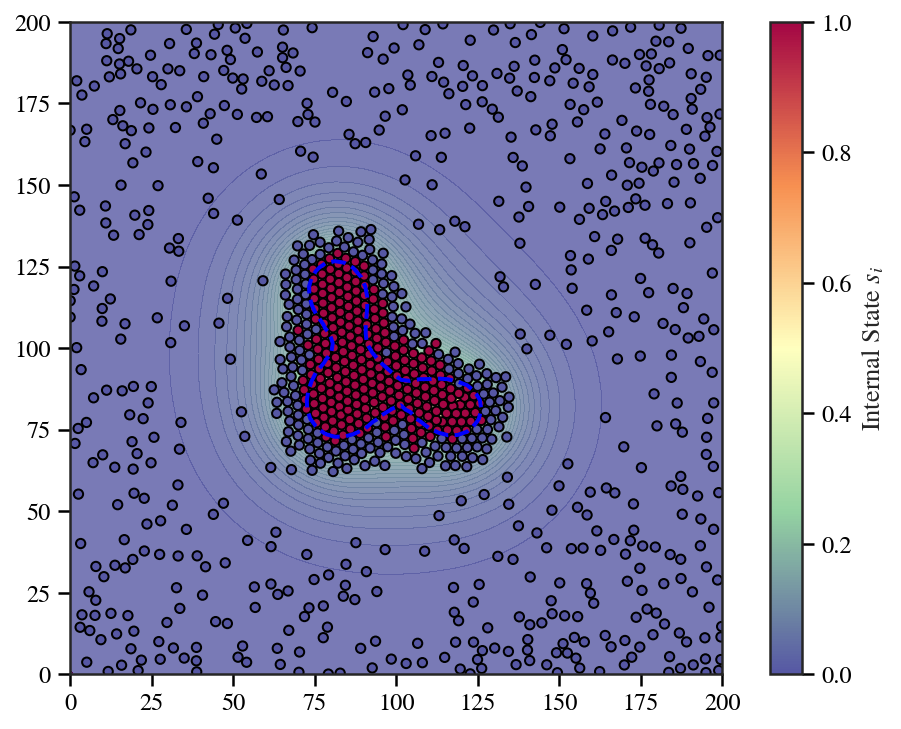
\includegraphics[width=\linewidth]{figs/simpleModeling3.png}
%     }
%     \hfill
%     \subcaptionbox{Final snapshot of only chimical fields}[0.49\linewidth]{
%       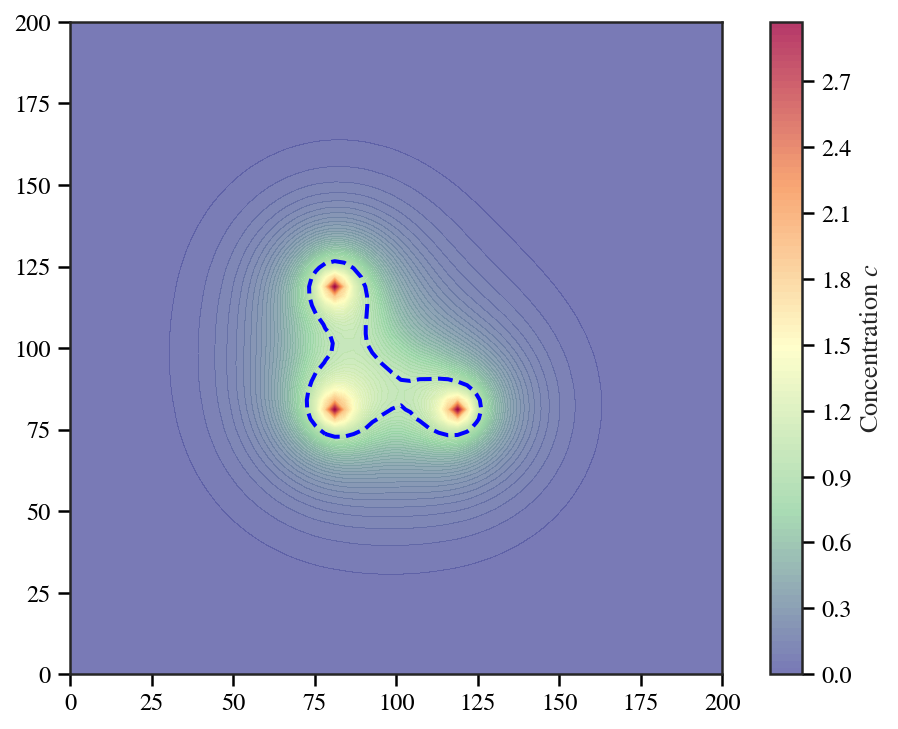
\includegraphics[width=\linewidth]{figs/simpleModeling4.png}
%     }
%     \caption{
%         The simulation of the model \eqref{eq:furtherModel} with $\alpha_c=-1$, $D_c=3$, $k_c=0.005$ and $\beta_c=0.1$. The blue dashed line is critical contour of the network region.
%         \textbf{(a)}, the particles are attracted to the target nodes and form a connected network like letter "L". The color of the particles represents their internal state $s_i$, with red indicating a high state and blue indicating a low state.
%         \textbf{(b)}, the chemical field is shown with the critical contour (blue dashed line) of the network region. It can be noticed that the critical contour lines obtained from $c$ are not a regular L-shape, but rather a short Y-shape, which is obviously more economic than the L-shape.
%     }
% \end{figure}

The above model have initially realized the network formation, but it does not solve the problem when the distance between nodes is large. To address this, we introduce a convection term $\mathbf{v}\cdot \nabla c$ in the chemical equation, which represents the influence of the particles' active transport on the chemical field. The updated model is as follows:
\begin{subequations}
    \begin{align}
        &\dot{\mathbf{r}}_i\left( t \right) =\alpha _c\nabla c-\nabla _{\mathbf{r}_i}V+\sqrt{2D_p}\boldsymbol{\eta }_i\;,\\
        &\dot{c}\left( \mathbf{r},t \right) =D_c\nabla ^2c-\mathbf{v}\cdot \nabla c-k_c c+\beta _c\sum\nolimits_j^{}{\delta \left( \mathbf{r}-\mathbf{r}_{j}^{*} \right) }\;,
    \end{align}
\end{subequations}
where $\mathbf{v}=v_{\boldsymbol{c}}\sum_{i=1}^N{\delta \left( \mathbf{r}-\mathbf{r}_i \right)\left( \cos \phi _{\mathbf{r}}, \sin \phi _{\mathbf{r}} \right) ^{\top}}$ is the convection velocity of the chemical field, $v_{\boldsymbol{c}}$ is the convection speed, and 
\begin{equation}
    \phi _{\mathbf{r}}= \tan^{-1} \left( \frac{y_{\mathrm{cm}}-y_i}{x_{\mathrm{cm}}-x_i} \right)
\end{equation}
is the angle toward the particle's center of mass at position $\mathbf{r}$, where $\left( x_{\mathrm{cm}},y_{\mathrm{cm}} \right) ^{\top}=N^{-1}\sum\nolimits_i^{}{\mathbf{r}_i}$.


\begin{subequations}
    \begin{align}
        &\mathbf{\dot{r}}_i\left( t \right) =\alpha _c\nabla c-\nabla _{\mathbf{r}_i}V+\sqrt{2D_p}\boldsymbol{\eta }_i\;,
        \\
        &\dot{c}\left( \mathbf{r},t \right) =D_c\nabla ^2c-k_cc+\sum\nolimits_j^{}{s_j\delta \left( \mathbf{r}-\mathbf{r}_{j}^{*} \right)}\;,
        \\
        &\dot{s}_j\left( t \right) =\left( 1+s_j \right) \left( 1-s_j \right) \left( s_{\text{th}}-\sum\nolimits_i^{}{\delta \left( \mathbf{r}_i-\mathbf{r}_{j}^{*} \right)} \right) 
    \end{align}
\end{subequations}


% \subsection{Final Definitions}
% We consider a 2D box with $N$ chemotactic particles and $M$ food source nodes. The particles are subject to a chemotactic force, a short-range repulsion force, and a noise term. The chemical concentration field evolves via diffusion, decay, and production from the target nodes, while each particle’s internal state regulates the local chemical concentration. 
% The dynamics are governed by the following equations:
% \begin{subequations}
%     \begin{align}
%         &\dot{\mathbf{r}}_i\left( t \right) =\alpha _c\nabla c-\nabla _{\mathbf{r}_i}V+\sqrt{2D_p}\boldsymbol{\eta }_i \;,
%         \\
%         &\dot{s}_i\left( t \right) =s_i\left( 1-s_i \right) \left( c_{\mathbf{r}_i}-c_s \right) \;,
%         \\
%         &\dot{c}\left( \mathbf{r},t \right) = D_c\nabla ^2c-k_c\left( 1-s_{\mathbf{r}} \right) c+\beta _c\sum\nolimits_j^{}{\delta \left( \mathbf{r}-\mathbf{r}_{j}^{*} \right)} \;,
%     \end{align}
%     \label{eq:finalModel}
% \end{subequations}
% for $i=1,2,\cdots,N$ and $j=1,2,\cdots,M$. Here, $\mathbf{r}_i$ and $\mathbf{r}_j^*$ denote the positions of the $i$-th particle and $j$-th node, respectively, $c$ is the concentration of chemical released by nodes, $\alpha _c<0$ is the chemotactic sensitivity, $V$ is the potential field of short-range repulsion, $D_p$ is the intensity of thermal noise, $s_i$ is the internal state of the $i$-th particle, $c_{\mathbf{r}_i}=c\left( \mathbf{r}_i\left( t \right) ,t \right) $ is the local chemical concentration at the position of the $i$-th particle, $D_c$ and $k_c$ are the diffusion coefficient and decay rate of the chemical, $s_{\mathbf{r}}=\sum\nolimits_i^{}{s_i\delta \left( \mathbf{r}-\mathbf{r}_i \right)}$ aggregates the internal states of particles at $\mathbf{r}$ (zero if no particle exists there), $\beta _c$ is the saturation concentration preventing unbounded growth. 
% The term $s_i\in \left[ 0,1 \right]$ and the repulsive interaction $\nabla _{\mathbf{r}_i}V$ ensure at most one particle occupies any position $\mathbf{r}$. Thus, $s_{\mathbf{r}} \leqslant 1$, guaranteeing the decay term $-k_c\left( 1-s_{\mathbf{r}} \right) c$ remains non-positive. In other words, particles modulate the chemical decay rate but do not contribute to its production, which is solely driven by the nodes.

\section{Behaviors}

\section{Continuum model}



\bibliography{ref}

\end{document}